\frame
{	\frametitle{Inhalt}
	\begin{itemize}
		\item Umsetzung der 3D-dimensionalen Fast-Fourier-Transformation in Multi-Prozessorsystemen in einem High-Performance-Computing Kontext
		\item algorithmische Methoden
		\item Beschleunigung durch Hardware
		\item Probleme bei der Umsetzung auf einer Multi-Prozessor-Systemarchitektur
	\end{itemize}
}

\frame
{
	\begin{center}
		\Large Fast Fourier Transformation \normalsize
	\end{center}
}

\frame
{
	\frametitle{FFT}
	\begin{figure}[h!]
		\centering
		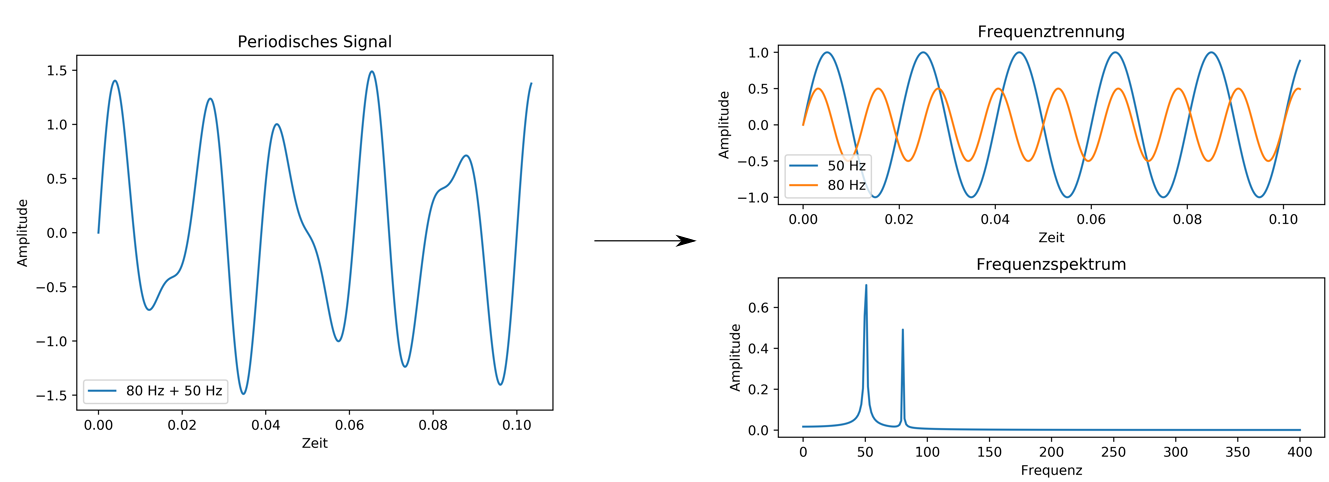
\includegraphics[width=\linewidth, keepaspectratio]{../Pictures/Fourierreihe.png}
	\end{figure}
	\begin{itemize}
		\item Algorithmus für diskrete Fourier Transformation (DFT)
		\item Transformation zeitdisretes periodisches Signal zu Frequenzspektrum 
		\item Anwendung in Natursimulationen, machinellem Lernen, Ingenieurswesen oder Signalmodulation
	\end{itemize}
}

\frame
{
	\frametitle{DFT}
	\begin{equation*}
		X_{k}= \sum_{n=0}^{N-1} x_{n} e^{-i2 \pi kn /N} \text{  für } k=0,...,N-1
	\label{eq:DFT}
	\end{equation*}
	\begin{itemize}
		\item zeitdiskretes Signal $x_{n} = x_{1}, x_{2},...$
		\item periodisches Frequenzspektrum $X_{k} = X_{1}, X_{2},...$
		\item Umformen mit der Einheitswurzel $w_{N} = e^{-2 \pi ik /N}$
	\end{itemize}
	
	\begin{equation*}
		X_{k}= \sum_{n=0}^{N-1} x_{n} w_{N}^{kn}
	\end{equation*}
}

\frame
{
	\frametitle{DFT Fouriermatrix}
	\begin{itemize}
		\item DFT mit Fouriermatrix $F_{N} = (w^{kn})_{k,n=0}^{N-1}$:
	\end{itemize}
	\vspace{5mm}
	\begin{equation*}
	X_{k} = x_{n}F_{N}
	\label{eq:dft fouriermatrix}
	\end{equation*}
	\vspace{3mm}
	\begin{equation*}
	\left( \begin{array}{cccc}
	w^0 & w^0 & \cdots & w^0\\
	w^0 & w^1 & \cdots & w^{N-1}\\
	\vdots & \vdots & \ddots & \vdots\\
	w^0 & w^{N-1} & \cdots & w^{(N-1)(N-1)}\\
	\end{array}\right)
	\left( \begin{array}{c}
	x_0\\
	x_1\\
	\vdots\\
	x_{N-1}
	\end{array}\right)
	\end{equation*}
}

\frame
{
	\frametitle{Implementierung FFT}
	\begin{itemize}
		\item Teile-Herrsche-Verfahren
		\item Aufteilung der Matrixmultiplikation mit $N$ Elementen auf zwei Matrixmultiplikationen mit $\frac{N}{2}$ Elementen
		\item Wiederholen bis 1 Element in der Matrix übrig bleibt
		\item $N$ ist Zweierpotenz
		\item Aufteilung der Matrix mit folgenden Eigenschaften:
		\begin{itemize}
			\item $w^{N/2} = -1$ \text{ für $N$ gerade}
			\item $w^{kN} = 1$
		\end{itemize}
	\end{itemize}

}


\frame
{
	\frametitle{FFT Beispiel}
	\begin{itemize}
		\item Eigenschaft $w^{kN} = 1$ in Zeile 1, 3, 5 und 7
	\end{itemize}
	\vspace{1mm}
	\begin{equation*}
	\left( \begin{array}{cccccccc}
	w^{0} & w^{0} & w^{0} & w^{0} & w^{0} & w^{0} & w^{0} & w^{0}\\
	w^{0} & w^{1} & w^{2} & w^{3} & w^{4} & w^{5} & w^{6} & w^{7}\\
	w^{0} & w^{2} & w^{4} & w^{6} & w^{8} & w^{10} & w^{12} & w^{14}\\
	w^{0} & w^{3} & w^{6} & w^{9} & w^{12} & w^{15} & w^{18} & w^{21}\\
	w^{0} & w^{4} & w^{8} & w^{12} & w^{16} & w^{20} & w^{24} & w^{28}\\
	w^{0} & w^{5} & w^{10} & w^{15} & w^{20} & w^{25} & w^{30} & w^{35}\\
	w^{0} & w^{6} & w^{12} & w^{18} & w^{24} & w^{30} & w^{36} & w^{42}\\
	w^{0} & w^{7} & w^{14} & w^{21} & w^{28} & w^{35} & w^{42} & w^{49}\\
	\end{array} \right)
\end{equation*}
}

\frame
{
	\frametitle{FFT Beispiel}
	\begin{itemize}
		\item Eigenschaft $w^{kN} = 1$ in Zeile 2, 4, 6 und 8
	\end{itemize}
	\vspace{1mm}
	\begin{equation*}
	\left( \begin{array}{cccccccc}
	w^{0} & w^{0} & w^{0} & w^{0} & w^{0} & w^{0} & w^{0} & w^{0}\\
w^{0} & w^{1} & w^{2} & w^{3} & w^{4} & w^{5} & w^{6} & w^{7}\\
w^{0} & w^{2} & w^{4} & w^{6} & w^{0} & w^{2} & w^{4} & w^{6}\\
w^{0} & w^{3} & w^{6} & w^{9} & w^{12} & w^{15} & w^{18} & w^{21}\\
w^{0} & w^{4} & w^{8} & w^{12} & w^{0} & w^{4} & w^{8} & w^{12}\\
w^{0} & w^{5} & w^{10} & w^{15} & w^{20} & w^{25} & w^{30} & w^{35}\\
w^{0} & w^{6} & w^{12} & w^{18} & w^{0} & w^{6} & w^{12} & w^{18}\\
w^{0} & w^{7} & w^{14} & w^{21} & w^{28} & w^{35} & w^{42} & w^{49}\\
	\end{array} \right)
\end{equation*}
}

\frame
{
	\frametitle{FFT Beispiel}
	\begin{itemize}
		\item Eigenschaft $w^{N/2} = -1$ in Zeile 2, 4, 6 und 8
	\end{itemize}
	\vspace{1mm}
	\begin{equation*}
	\left( \begin{array}{cccccccc}
	w^{0} & w^{0} & w^{0} & w^{0} & w^{0} & w^{0} & w^{0} & w^{0}\\
w^{0} & w^{1} & w^{2} & w^{3} & w^{4} & w^{5} & w^{6} & w^{7}\\
w^{0} & w^{2} & w^{4} & w^{6} & w^{0} & w^{2} & w^{4} & w^{6}\\
w^{0} & w^{3} & w^{6} & w^{9} & w^{4} & w^{7} & w^{10} & w^{13}\\
w^{0} & w^{4} & w^{8} & w^{12} & w^{0} & w^{4} & w^{8} & w^{12}\\
w^{0} & w^{5} & w^{10} & w^{15} & w^{4} & w^{9} & w^{14} & w^{19}\\
w^{0} & w^{6} & w^{12} & w^{18} & w^{0} & w^{6} & w^{12} & w^{18}\\
w^{0} & w^{7} & w^{14} & w^{21} & w^{4} & w^{11} & w^{18} & w^{25}\\
	\end{array} \right)
\end{equation*}
}

\frame
{
	\frametitle{FFT Beispiel}
	\begin{equation*}
	\left( \begin{array}{cccccccc}
		w^{0} & w^{0} & w^{0} & w^{0} & w^{0} & w^{0} & w^{0} & w^{0}\\
w^{0} & w^{1} & w^{2} & w^{3} & -w^{0} & -w^{1} & -w^{2} & -w^{3}\\
w^{0} & w^{2} & w^{4} & w^{6} & w^{0} & w^{2} & w^{4} & w^{6}\\
w^{0} & w^{3} & w^{6} & w^{9} & -w^{0} & -w^{3} & -w^{6} & -w^{9}\\
w^{0} & w^{4} & w^{8} & w^{12} & w^{0} & w^{4} & w^{8} & w^{12}\\
w^{0} & w^{5} & w^{10} & w^{15} & -w^{0} & -w^{5} & -w^{10} & -w^{15}\\
w^{0} & w^{6} & w^{12} & w^{18} & w^{0} & w^{6} & w^{12} & w^{18}\\
w^{0} & w^{7} & w^{14} & w^{21} & -w^{0} & -w^{7} & -w^{14} & -w^{21}\\
	\end{array} \right)
\end{equation*}
}

\frame
{
	\frametitle{FFT Beispiel}
	\begin{equation*}
	\left( \begin{array}{*{8}{@{}c}@{}}
w^{0} & w^{0} & w^{0} & w^{0} & w^{0} & w^{0} & w^{0} & w^{0}\\
w^{0}w^{0} & w^{1}w^{0} & w^{2}w^{0} & w^{3}w^{0} & -w^{0}w^{0} & -w^{1}w^{0} & -w^{2}w^{0} & -w^{3}w^{0}\\
w^{0} & w^{2} & w^{4} & w^{6} & w^{0} & w^{2} & w^{4} & w^{6}\\
w^{0}w^{0} & w^{1}w^{2} & w^{2}w^{4} & w^{3}w^{6} & -w^{0}w^{0} & -w^{1}w^{2} & -w^{2}w^{4} & -w^{3}w^{6}\\
w^{0} & w^{4} & w^{8} & w^{12} & w^{0} & w^{4} & w^{8} & w^{12}\\
w^{0}w^{0} & w^{1}w^{4} & w^{2}w^{8} & w^{3}w^{12} & -w^{0}w^{0} & -w^{1}w^{4} & -w^{2}w^{8} & -w^{3}w^{12}\\
w^{0} & w^{6} & w^{12} & w^{18} & w^{0} & w^{6} & w^{12} & w^{18}\\
w^{0}w^{0} & w^{1}w^{6} & w^{2}w^{12} & w^{3}w^{18} & -w^{0}w^{0} & -w^{1}w^{6} & -w^{2}w^{12} & -w^{3}w^{18}\\
	\end{array} \right)
\end{equation*}
}

\frame
{
	\frametitle{FFT Beispiel}
	\begin{equation*}
	\left( \begin{array}{*{8}{@{}c}@{}}
w^{0} & w^{0} & w^{0} & w^{0} & w^{0} & w^{0} & w^{0} & w^{0}\\
w^{0}w^{0} & w^{1}w^{0} & w^{2}w^{0} & w^{3}w^{0} & -w^{0}w^{0} & -w^{1}w^{0} & -w^{2}w^{0} & -w^{3}w^{0}\\
w^{0} & w^{2} & w^{4} & w^{6} & w^{0} & w^{2} & w^{4} & w^{6}\\
w^{0}w^{0} & w^{1}w^{2} & w^{2}w^{4} & w^{3}w^{6} & -w^{0}w^{0} & -w^{1}w^{2} & -w^{2}w^{4} & -w^{3}w^{6}\\
w^{0} & w^{4} & w^{8} & w^{12} & w^{0} & w^{4} & w^{8} & w^{12}\\
w^{0}w^{0} & w^{1}w^{4} & w^{2}w^{8} & w^{3}w^{12} & -w^{0}w^{0} & -w^{1}w^{4} & -w^{2}w^{8} & -w^{3}w^{12}\\
w^{0} & w^{6} & w^{12} & w^{18} & w^{0} & w^{6} & w^{12} & w^{18}\\
w^{0}w^{0} & w^{1}w^{6} & w^{2}w^{12} & w^{3}w^{18} & -w^{0}w^{0} & -w^{1}w^{6} & -w^{2}w^{12} & -w^{3}w^{18}\\
	\end{array} \right)
	\left( \begin{array}{cccccccc}
x_1\\
x_2\\
x_3\\
x_4\\
x_5\\
x_6\\
x_7\\
x_8\\
\end{array} \right)
\end{equation*}
}


\frame
{
	\frametitle{FFT Beispiel}
	\begin{equation*}
	\left( \begin{array}{cccc}
w^{0} & w^{0} & w^{0} & w^{0}\\
w^{0} & w^{2} & w^{4} & w^{6}\\
w^{0} & w^{4} & w^{8} & w^{12}\\
w^{0} & w^{6} & w^{12} & w^{18}\\
\end{array} \right)
\left( \begin{array}{cccc}
x_1 + x_5\\
x_2 + x_6\\
x_3 + x_7\\
x_4 + x_8\\
\end{array} \right)
\end{equation*}
\begin{equation*}
\left( \begin{array}{cccc}
w^{0} & w^{0} & w^{0} & w^{0}\\
w^{0} & w^{2} & w^{4} & w^{6}\\
w^{0} & w^{4} & w^{8} & w^{12}\\
w^{0} & w^{6} & w^{12} & w^{18}\\
\end{array} \right)
\left( \begin{array}{cccc}
w^{0}(x_1 - x_5)\\
w^{1}(x_2 - x_6)\\
w^{2}(x_3 - x_7)\\
w^{3}(x_4 - x_8)\\
\end{array} \right)
\end{equation*}
}

\frame
{
	\frametitle{FFT Beispiel}
	\begin{figure}[h!]
		\centering
		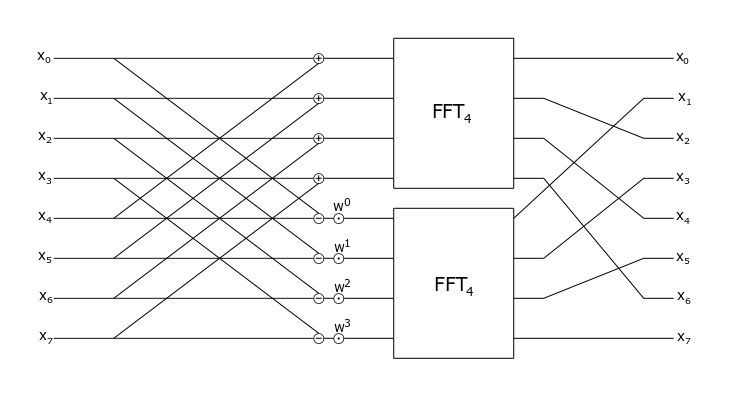
\includegraphics[width=\linewidth, keepaspectratio]{../Pictures/FFTPres.png}
	\end{figure}
	
}


\frame
{
	\frametitle{3D-FFT}
	\begin{figure}[h!]
		\centering
		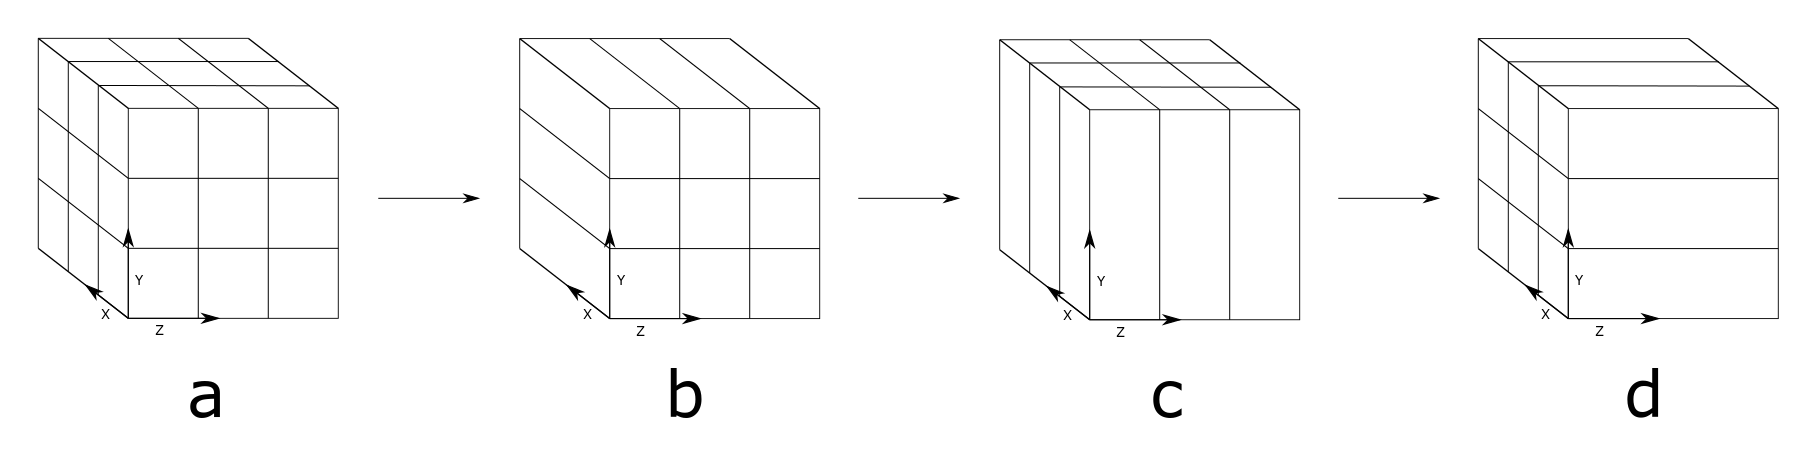
\includegraphics[width=\linewidth, keepaspectratio]{../Pictures/PencilsDecompositionPres.png}
	\end{figure}
	\begin{itemize}
		\item Aufteilung in 3 seperate 1D-FFTs
		\item Umformen der Daten in sogenannte Pencils
		\item Aufteilen der Pencils auf die Prozesse
		\item Berechnen der 1D-FFTs
	\end{itemize}
		
	
}

